\chapter{Performance Degradation}

\vspace{-0.3em}

\section{Evaluation Metric: ROC-AUC}

We used the \textbf{Area under the Reciever Operating Characteristic Curve} (\textbf{ROC-AUC}) to evaluate model performance. The \textbf{ROC} plots the true positive rate against the false positive rate and ranges from 0 to 1, with higher values indicating better model performance.

Because the AUC focuses on how well the model ranks positive instances above negative ones, it is generally more robust to imbalanceness in data distributions rather than metrics like accuracy.

\vspace{-0.3em}

\section{Evaluated models}

As metioned in the first chapter, simple covariate shift can lead to serious degradations in model performance. In this chapter, we will analyze how different statistical learning models' performances are affected by covariate shift. 

We evaluated a diverse set of models to comprehensively assess their robustness under covariate shift conditions:

\begin{itemize}
    \item \textbf{Logistic Regression}: A generalised linear model that serves as a baseline model;
    \item \textbf{Random Forest}: An ensemble learning method that builds multiple decision trees and averages their predictions to improve performance;
    \item \textbf{Gradient Boosting}: An ensemble learning method that builds sequential weak learners (in our case decision trees) to correct prediction errors iteratively, focusing on residuals from previous predictions;
    \item \textbf{eXtreme Gradient Boosting (XGBoost)}: A highly optimized implementation of gradient boosting machines known for its efficiency and performance.
\end{itemize}

As we will see, these models (except the logistic regression) have different hyperparameters that can be tuned to improve performance. We used a grid search with 5-fold cross-validation to find the best hyperparameters for each model.

\vspace{-0.2em}

\begin{tcolorbox}[colback=gray!10,colframe=gray!70,title= What are Grid Search and Cross Validation?]
	\textbf{Grid Search} is a hyperparameter optimization technique that systematically searches through a fixed grid of hyperparameters with a brute-force method that evaluates all possible combinations of hyperparameters to find the best model.

	\vspace{0.3em}

	\textbf{Cross-validation} is a technique used to evaluate the performance of a model by splitting the data into $k$ subsets (folds) and training the model on $k-1$ folds while using the remaining fold for validation. This process is repeated $k$ times, with each fold used once as a validation set.
	
	\vspace{0.3em}

	\underline{\textbf{Note}}: This method only uses training data to optimize hyperparameters, reflecting real scenarios where test data is unavailable during training.
\end{tcolorbox}

\subsection{Logistic Regression}

Logistic regression models the relationship between features and the target variable using linear combinations of the input variables, which may not capture complex nonlinear patterns in the data. Given the assumed nonlinear relationships between variables, which also includes intersactions, we decided to use as baseline model the one including all the interaction terms (\texttt{X1:X2}, \texttt{X1:X3}, \texttt{X2:X3}, and \texttt{X1:X2:X3}).

We used the \texttt{statsmodels} library to fit a logistic regression model on the training dataset and evaluated it on the test set. The table below summarizes the coefficients, significance (\textit{P>|z|}), and confidence intervals for the fitted logistic regression baseline model.

\vspace{0.5em}

\begin{table}[H]
    \small
    \centering
    \begin{tabular}{lrrrrrr}
        \toprule
        & \textbf{coef} & \textbf{std err} & \textbf{z} & \textbf{P>|z|} & \textbf{[0.025} & \textbf{0.975]} \\
        \midrule
        \textbf{Intercept} & \textcolor{red}{-0.9761} & 0.122 & -8.022 & 0.000 & -1.215 & -0.738 \\
        \textbf{X1}        & \textcolor{red}{-0.6550} & 0.120 & -5.462 & 0.000 & -0.890 & -0.420 \\
        \textbf{X2}        & -0.2049 & 0.180 & -1.139 & 0.255 & -0.558 & 0.148 \\
        \textbf{X1:X2}     & \textcolor{red}{-0.2653} & 0.125 & -2.118 & 0.034 & -0.511 & -0.020 \\
        \textbf{X3}        & \textcolor{red}{1.3187}  & 0.115 & 11.478 & 0.000 & 1.094  & 1.544 \\
        \textbf{X1:X3}     & \textcolor{red}{1.3248}  & 0.106 & 12.453 & 0.000 & 1.116  & 1.533 \\
        \textbf{X2:X3}     & -0.3253 & 0.172 & -1.894 & 0.058 & -0.662 & -0.011 \\
        \textbf{X1:X2:X3}  & 0.0510  & 0.120 & 0.427  & 0.670 & -0.183 & 0.285 \\
        \bottomrule
    \end{tabular}
    \caption{\quad \textbf{Summary of Logistic Regression coefficients.} \newline
	Coefficients with statistical significance ($p < 0.05$) are hilighted in red.}
    \label{tab:regression_results}
\end{table}

As we can see from the table, for this data instance, the features $X_2$, $X_2:X_3$ and $X_1:X_2:X_3$ are not statistically significant, as their p-values are above the 0.05 threshold. This suggests that these features may not be relevant for predicting the target variable $Y$, but bare in mind that this is only one instance of the data and the results may vary across different instances.

The following plots show the ROC curves and the AUC scores for the logistic regression model under different levels of covariate shift.

\vspace{0.2em}

\begin{figure}[H]
	\centering
	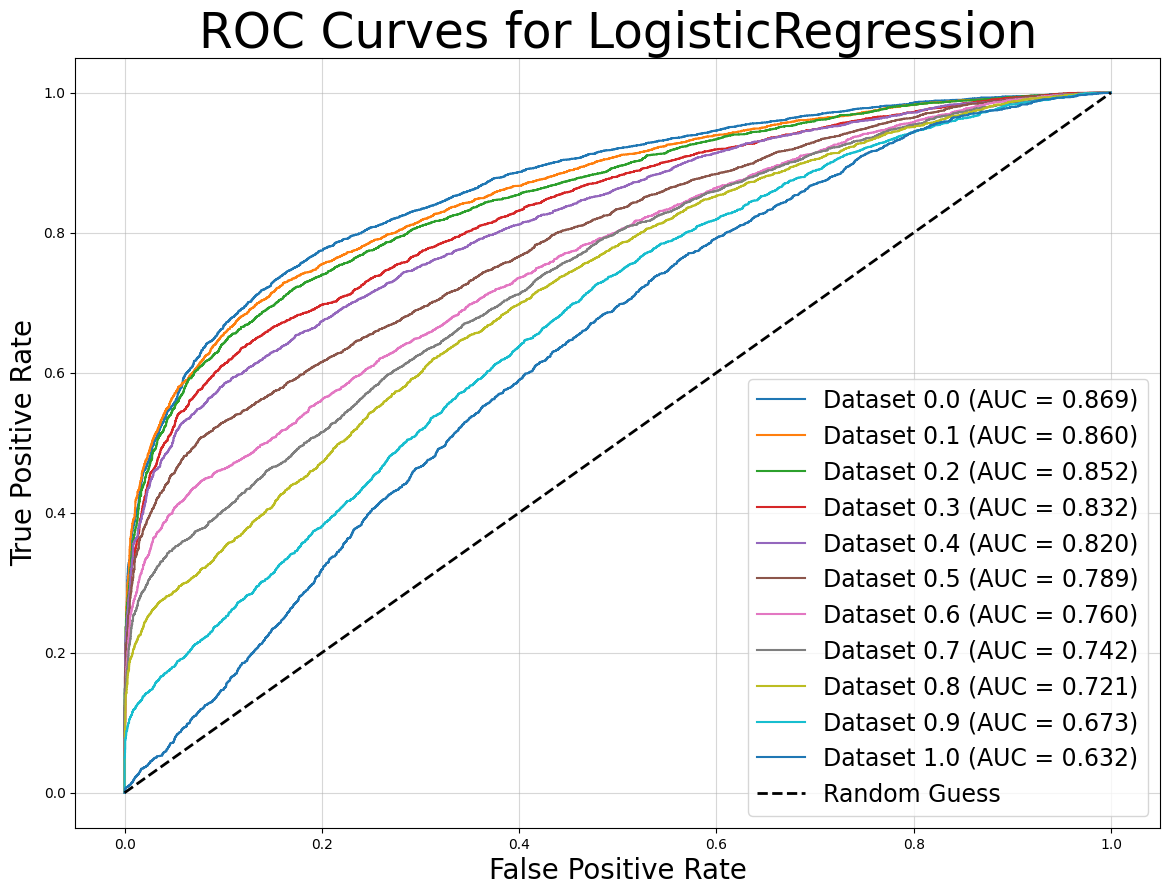
\includegraphics[width=0.65\textwidth]{assets/lr_auc.png}
	\caption{\textbf{Performance of the Logistic Regression model under covariate shift.} \newline The AUC scores of the model are plotted against the mixing probability $p$, which represents the proportion of shifted data in the test set.}
	\label{fig:logistic-regression-perf}
\end{figure}

\subsection{Ranfom Forests}

Random Forests are an ensemble learning technique that constructs multiple independent decision trees and combines their outputs through averaging to enhance predictive accuracy.

We used the \texttt{RandomForestClassifier} from the \texttt{scikit-learn} library. This model presents several hyperparameters that can be tuned to improve performance. To find the best hyperparameters we used the \texttt{scikit-learn} \texttt{GridSearchCV} method with 5-fold cross-validation.

The best hyperparameters found are shown in the following table:

\vspace{0.3em}

\begin{table}[H]
    \centering
    \begin{tabular}{l|c}
    \toprule
    \textbf{Parameter} & \textbf{Value} \\
    \midrule
    n\_estimators & 125 \\
    criterion & gini \\
    max\_depth & 6 \\
    min\_samples\_leaf & 1 \\
    min\_samples\_split & 5 \\
    bootstrap & True \\
    \bottomrule
    \end{tabular}
    \label{tab:rf_hyperparameters}
    \caption{Best hyperparameters found for the Random Forest model using 5-fold cross validation}
\end{table}

We also used a fixed \texttt{random\_state=0} to ensure reproducibility of results.

The following plot shows the ROC curves and the AUC scores for the Random Forest model under different levels of covariate shift.

\vspace{0.5em}

\begin{figure}[H]
	\centering
	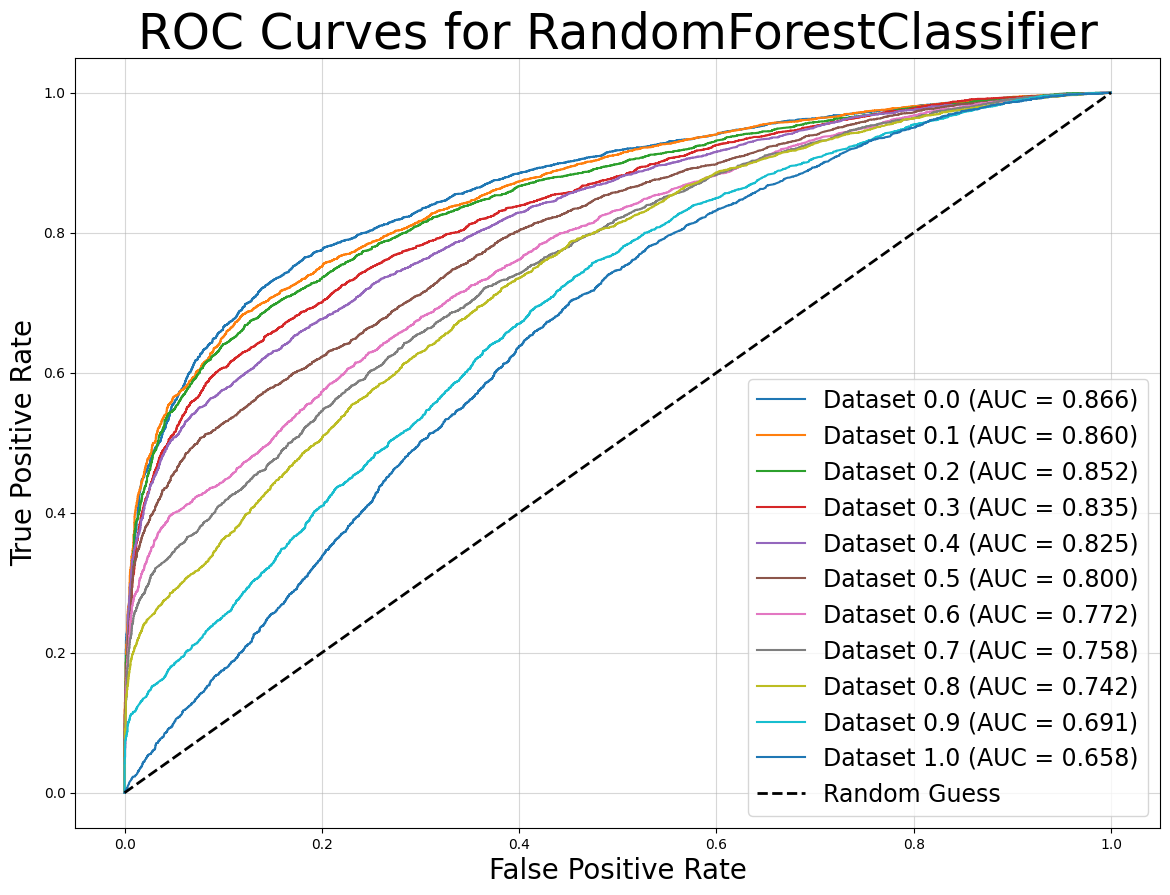
\includegraphics[width=0.65\textwidth]{assets/rf_auc.png}
	\caption{\textbf{Performance of the Random Forest model under covariate shift.} \newline The AUC scores of the model are plotted against the mixing probability $p$, which represents the proportion of shifted data in the test set.}
	\label{fig:random-forest-perf}
\end{figure}

\newpage

\subsection{Gradient Boosting}

Gradient Boosting builds sequential weak learners (in our case decision trees) to iteratively correct prediction errors by focusing on residuals from previous predictions. Unlike Random Forests where trees are built independently, each tree in Gradient Boosting learns from the mistakes of previous trees.

We used \texttt{scikit-learn}'s \texttt{GradientBoostingClassifier}. Also in this case we used \texttt{GridSearchCV} method from \texttt{scikit-learn} library with a 5-fold cross-validation to find the following optimized hyperparameters:

\vspace{0.3em}

\begin{table}[H]
	\centering
	\begin{tabular}{l|c}
		\toprule
		\textbf{Parameter} & \textbf{Value} \\
		\midrule
		n\_estimators & 500 \\
		learning\_rate & 0.005 \\
		max\_depth & 3 \\
		subsample & 0.4 \\
		\bottomrule
	\end{tabular}
	\caption{Best hyperparameters found for the Gradient Boosting model using 5-fold cross validation}
\end{table}

As with the Random Forest model, we used a fixed \texttt{random\_state=0} to ensure reproducibility of results.

The following plot shows the ROC curves and AUC scores under different levels of covariate shift:

\vspace{0.5em}

\begin{figure}[H]
	\centering
	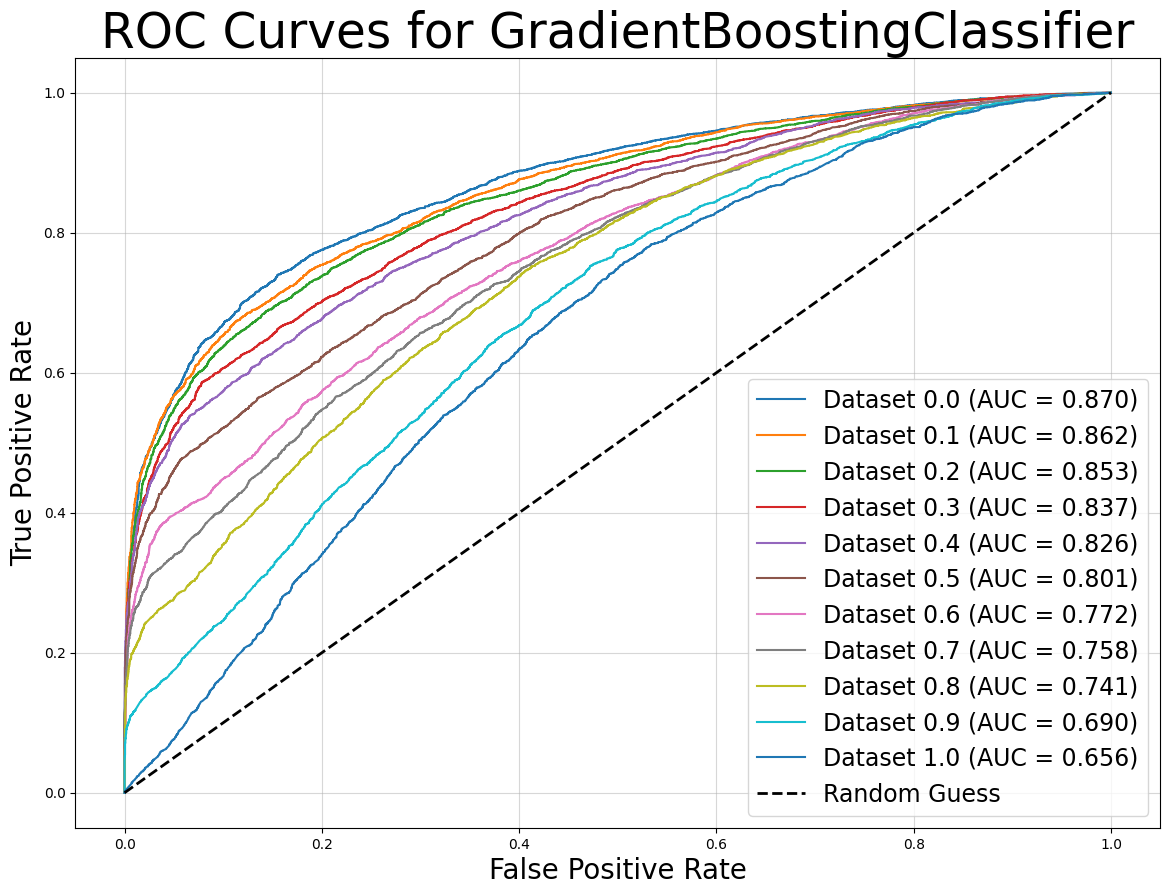
\includegraphics[width=0.65\textwidth]{assets/gbc_auc.png}
	\caption{\textbf{Performance of the Gradient Boosting model under covariate shift.} \newline The AUC scores are plotted against the mixing probability $p$, representing the proportion of shifted data in the test set.}
	\label{fig:gradient-boosting-perf}
\end{figure}

\newpage

\subsection{XGBoost}

XGBoost (eXtreme Gradient Boosting) is an advanced implementation of gradient boosting machines that offers enhanced regularization to prevent overfitting and superior computational efficiency through parallel processing.

We used the \texttt{XGBoost} library's \texttt{XGBClassifier}.

Due to incompatibility between the \texttt{XGBoost} library and \texttt{scikit-learn}'s \texttt{GridSearchCV}, we implemented a \textbf{custom parallel grid search with 5-fold cross-validation}.

This custom implementation leverages XGBoost's native \textbf{multi-threading} capabilities and \textbf{GPU acceleration} to efficiently evaluate hyperparameter combinations across multiple processing cores, significantly reducing the computational time required for model optimization.

The best hyperparameters found are shown in the following table:

\vspace{0.3em}

\begin{table}[H]
	\centering
	\begin{tabular}{l|c}
	\toprule
	\textbf{Parameter} & \textbf{Value} \\
	\midrule
	n\_estimators & 100 \\
	learning\_rate & 0.1 \\
	max\_depth & 3 \\
	min\_child\_weight & 1 \\
	subsample & 0.8 \\
	colsample\_bytree & 0.8 \\
	\bottomrule
	\end{tabular}
	\caption{Best hyperparameters found for the XGBoost model using 5-fold cross validation}
\end{table}

The following plot shows the ROC curves and AUC scores under different levels of covariate shift:

\vspace{0.5em}

\begin{figure}[H]
	\centering
	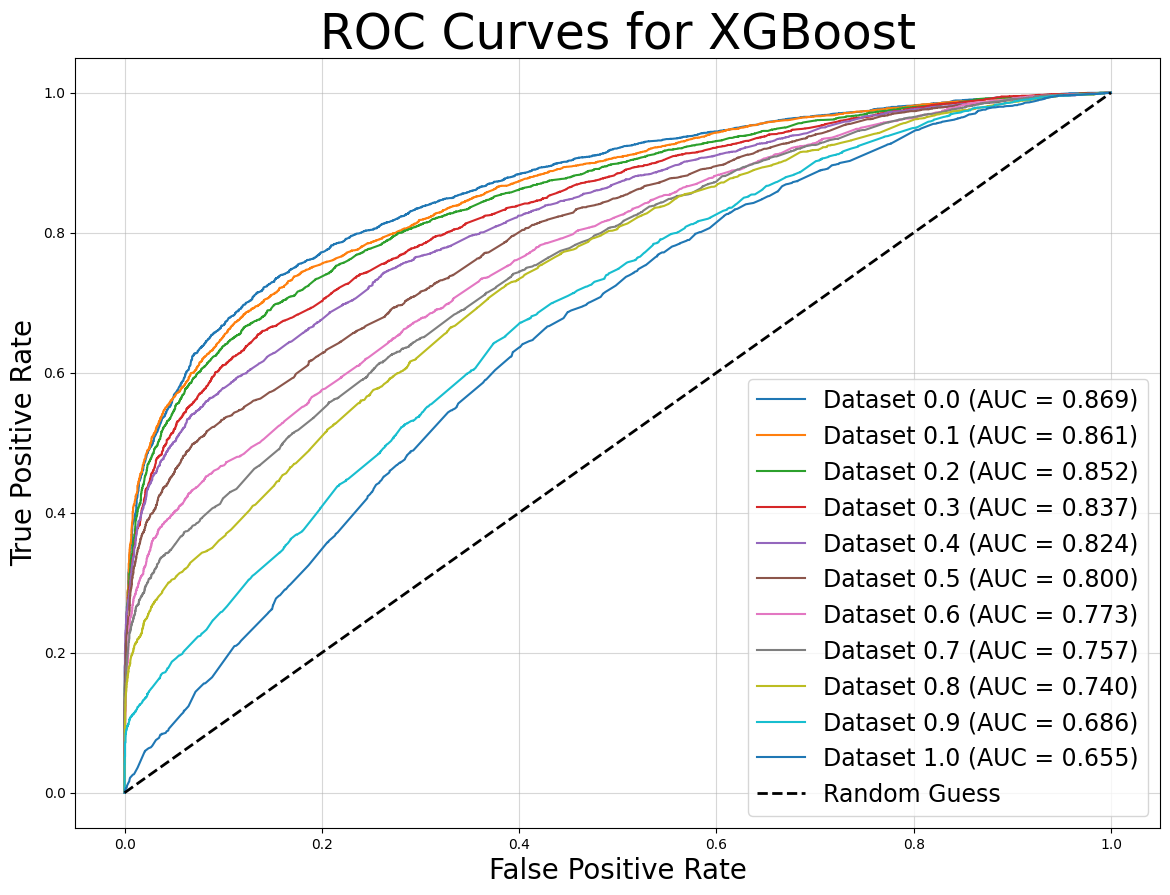
\includegraphics[width=0.65\textwidth]{assets/xgb_auc.png}
	\caption{\textbf{Performance of the XGBoost model under covariate shift.} \newline The AUC scores are plotted against the mixing probability $p$, representing the proportion of shifted data in the test set.}
	\label{fig:xgboost-perf}
\end{figure}

\section{Model Comparison}

\subsection{Preliminary Analysis}

The following plot shows the AUC scores of the fine-tuned models under different levels of covariate shift:

\begin{figure}[H]
    \centering
    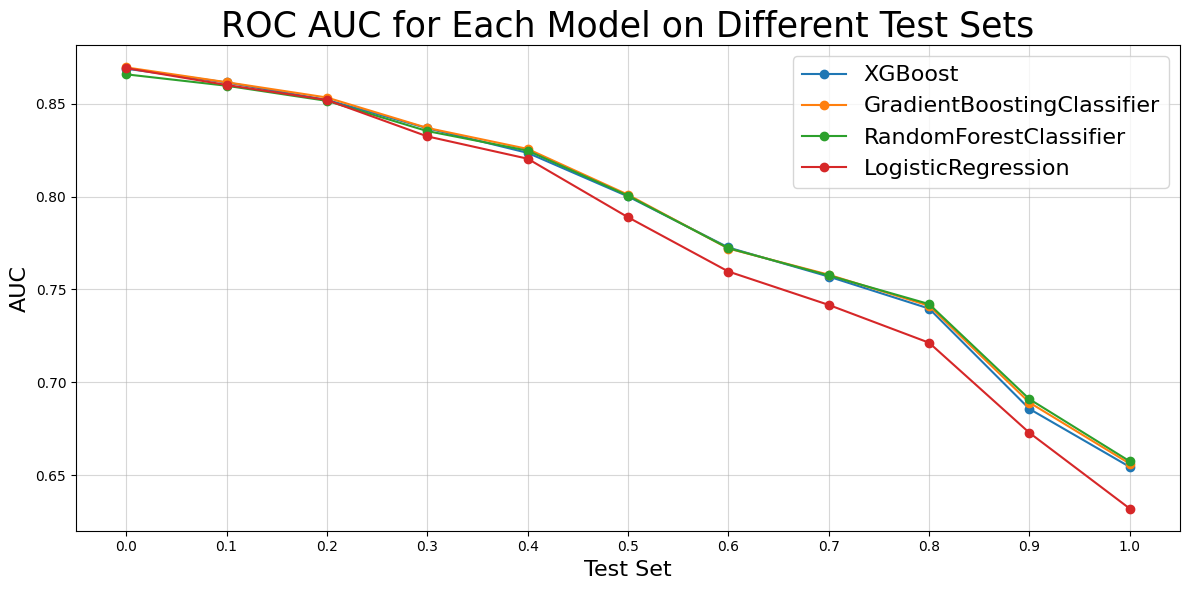
\includegraphics[width=0.8\textwidth]{assets/auc_comp.png} 
    \caption{\textbf{Performance comparison of fine tuned models under covariate shift.}}
    \label{fig:tuned-models-perf}
\end{figure}

As we can see from the plot, all the ensemble models (Random Forest, Gradient Boosting, and XGBoost) behaves very similarly under covariate shift, with a monotone decrease in performance as the mixing probability $p$ increases. The logistic regression model, on the other hand, shows a decrease in performance as the mixing probability increases. Notably, the model performs identically on datasets with statistical mixture probabilities ranging from 0\% to 20\%, showing the first signs of a performance decline starting at a 30\% mixture probability.

\subsection{Statistical Analysis}

To give statistical support to our study we repeated this experiment $N = 50$ times. Keeping always the same training set (in order to not train the models several times), for each repetition we 
defined a new shifted ditribution $\mathcal{N}(\boldsymbol{\mu}_{\text{shift}}, \boldsymbol{\Sigma}_{\text{shift}}) $;
created 11 \textbf{testing} datasets $\mathcal{D}_\alpha$ with $\alpha \in \{0.0, 0.1, \ldots, 1.0\}$, where $\alpha$ represents the mixing probability as before and finally computed the ROC-AUC score for each model on each testing dataset.

In \cref{fig:mean-boxplot}, the boxplots depict the 50 ROC-AUC values for each model, calculated by averaging the AUC scores across the 11 testing datasets for each mixing probability $\alpha$. As observed in the plot, all ensemble models exhibit comparable performance in terms of median values and interquartile range (IQR). Furthermore, all ensemble models demonstrate higher median values compared to the baseline logistic regression model. 

A similar trend is evident in \cref{fig:boxplot}, which presents the boxplots of the 50 ROC-AUC values for each model, focusing exclusively on datasets with a mixing probability of $\alpha = 1.0$ (fully shifted datasets). In this case, as expected, the overall performance deteriorates compared to the results in \cref{fig:mean-boxplot}. However, the difference between the median values of the ensemble models and the logistic regression model becomes even more pronounced (approximately $10\%$). 

In both scenarios, the ensemble models exhibit lower variability compared to the logistic regression model while producing very similar results among themselves. Interestingly, there are occasional instances where the logistic regression model achieves performance comparable to that of the ensemble models. This is likely attributable to the stochastic nature of the data generation process.

\vspace {2em}

\begin{figure}[H]
	\centering
	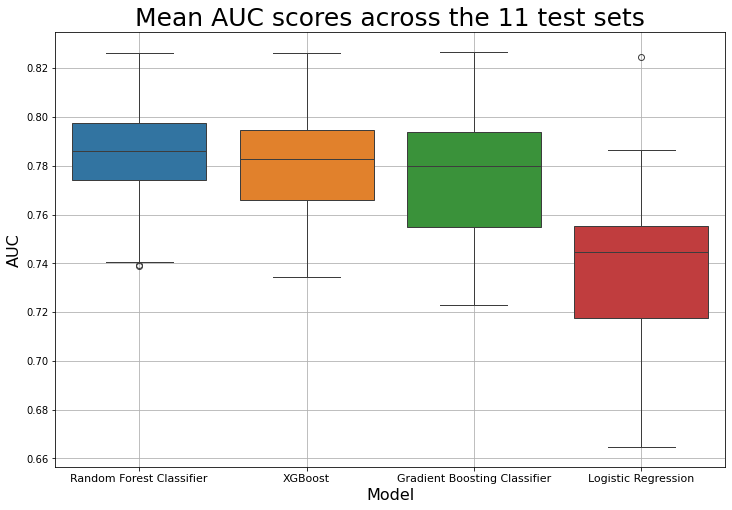
\includegraphics[width=0.8\textwidth]{assets/mean_boxplot.png} 
	\caption{\textbf{}}
	\label{fig:mean-boxplot}
\end{figure}

\vspace {2em}

\begin{figure}[H]
    \centering
    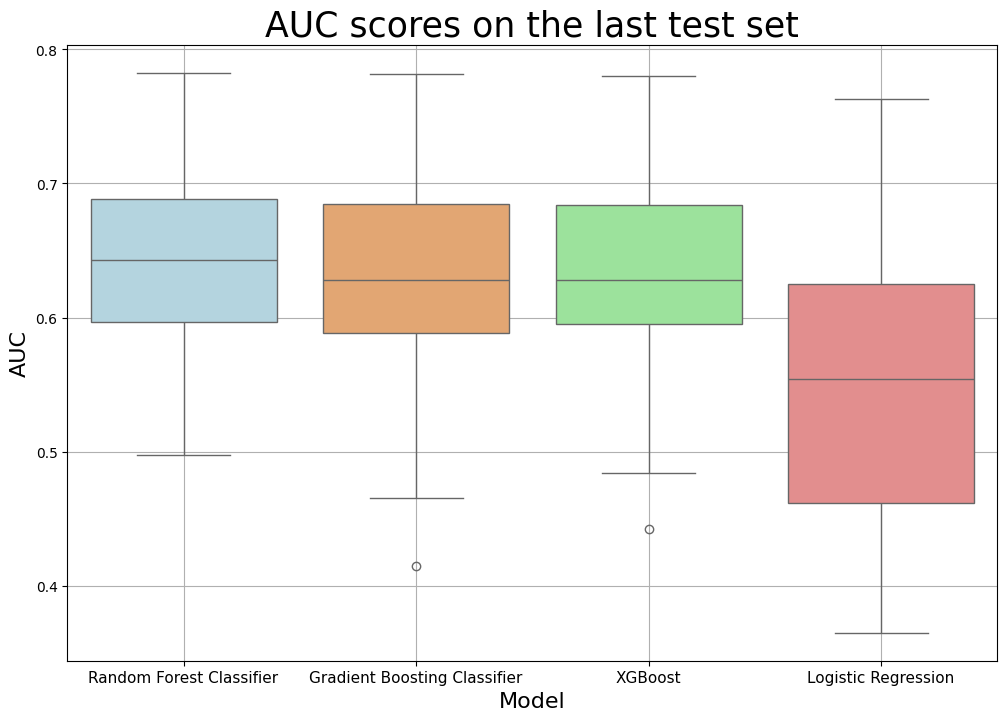
\includegraphics[width=0.8\textwidth]{assets/boxplot.png} 
    \caption{\textbf{}}
    \label{fig:boxplot}
\end{figure}


